\section{Marco teórico}

En esta sección, presentamos algunos términos, conceptos y teoremas que utilizaremos para construir el modelo matemático.

\subsection{Conceptos básicos}

La interacción de un objeto con las fuerzas que se ejercen sobre él se suele diagramar mediante un \textbf{diagrama de cuerpo libre} (DCL): ``un diagrama que muestra el cuerpo elegido solo, ``libre'' de su entorno, con vectores que muestren las magnitudes y direcciones de todas las fuerzas aplicadas sobre el cuerpo por todos los cuerpos que interactúan en él'' \citep{young}.

Por ejemplo, consideremos un objeto siendo arrastrado por el piso mediante una cuerda atada a un carro en movimiento. La figura \ref{fig:dcl-ejemplo} muestra esta situación y el DCL para este objeto siendo arrastrado.

\begin{figure}[ht!]
    \centering
    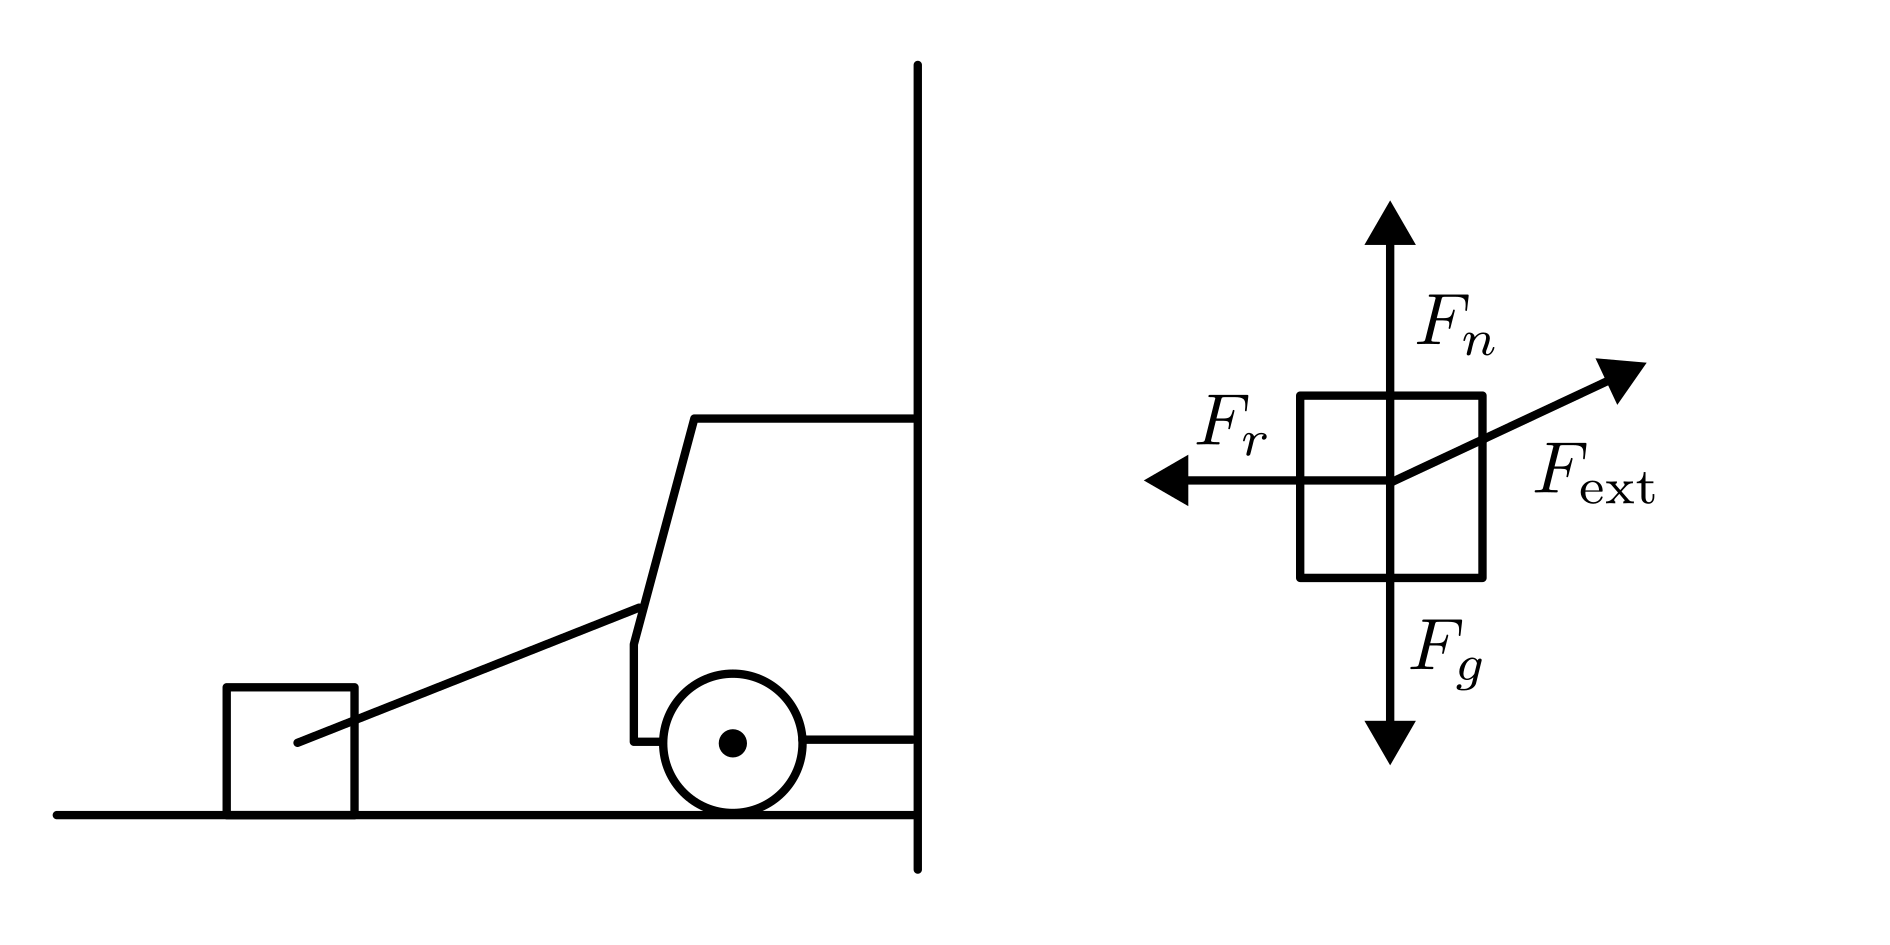
\includegraphics[width=0.6\textwidth]{dcl_ejemplo}
    \caption{Un ejemplo de sistema físico y el DCL de uno de sus elementos}
    \label{fig:dcl-ejemplo}
\end{figure}

\begin{definition}[amortiguamiento]
    En un sistema físico, el \textbf{amortiguamiento} (o amortiguación) es el fenómeno que ocurre en los objetos en movimiento, el cual \textit{disipa} la energía cinética.
\end{definition}

En sistemas físicos con velocidades relativamente bajas, se considera al amortiguamiento ejercido sobre un objeto como una fuerza proporcional y opuesta a su velocidad. \citet{rak} la definen mediante la relación
\[
    F_a = -cv
,\]
donde \(v\) es la velocidad del objeto (en \si{m/s}) y \(c\) es la \textbf{constante de amortiguamiento} (en \si{kg/s} y no negativa). Este tipo de amortiguamiento se denomina \textbf{amortiguamiento viscoso} \citep{rak}.

En la práctica, el amortiguamiento se suele definir mediante una \textbf{razón de amortiguamiento} (un coeficiente sin unidades), denotada por \(\zeta\). La constante de amortiguamiento \(c\) se puede calcular a partir la razón \(\zeta\) mediante
\[
    c = \zeta \left( 2\sqrt{mk} \right)
,\]
donde \(m\) es la masa del objeto y \(k\) su constante de elasticidad (concepto que será detallado más adelante en el marco teórico).

\subsection{Resultados y teoremas}

En primer lugar, es esencial para este trabajo enunciar la segunda ley de Newton, la cual parafraseamos del trabajo de \citet{young}.

\begin{theorem}[segunda ley de Newton]
    Sea \(m\) la masa (en \si{kg}) de un objeto, sea \(a\) su aceleración (en \si{m/s^2}) y sea \(\sum F_i\) (también llamada ``fuerza neta'') la suma de todas las fuerzas siendo aplicadas en dicho objeto en un instante particular.
    
        Entonces, en ese instante particular se cumple la ecuación
        \[
            \sum F_i = ma
        .\]
\end{theorem}

Esta ecuación será la base del modelo matemático que derivaremos.

La siguiente ley, también ampliamente conocida, nos permite caracterizar una de las fuerzas elásticas que actúan sobre las estructura que analizaremos más adelante. Parafraseando el trabajo de \citet{giuli}, enuncia lo siguiente:

\begin{theorem}[ley de Hooke]
    Sea \(x\) la posición (en metros) de un objeto con respecto a su punto de equilibrio, y sea \(F_e\) la \textbf{fuerza restauradora} ejercida sobre el objeto debido a su elasticidad.
    
        Entonces, se cumple que dicha fuerza restauradora es igual a
        \begin{equation}\label{eqn:hooke}
            F_{s} = -kx
        ,\end{equation}
        donde \(k\) (en \si{N/m}) es una constante no negativa llamada la \textbf{constante de elasticidad}.
\end{theorem}

En otras palabras, la fuerza restauradora ejercida sobre un objeto por elasticidad es proporcional a su posición con respecto a su punto de equilibrio.

En particular, \eqref{eqn:hooke} se puede aplicar al modelar la fuerza de restauración ejercida sobre una estructura que vibra horizontalmente, ya que se puede considerar que ``presenta un comportamiento elástico'' \citep{tarque}. En esta situación, se le llama a \(k\) la \textbf{rigidez} de la estructura.


\subsection{Métodos numéricos y Runge-Kutta}

Mientras que el modelado de fenómenos físicos por medio de ecuaciones diferenciales no es un proceso necesariamente complicado, su resolución a través de métodos analíticos exactos resulta, en muchos casos, una tarea muy difícil (o imposible). En este tipo de situaciones, los métodos numéricos son de gran utilidad para obtener soluciones aproximadas en lugar de analíticas \citep{reddy}.

Una familia de métodos numéricos que destacan por su simplicidad y efectividad son los métodos Runge-Kutta. Dentro de ellos, uno de los más frecuentemente usados es el método de \textbf{Runge-Kutta de orden 4} (RK4), el cual, parafraseando a \citet{suli}, consiste en aproximar iterativamente una EDO de la forma
\[
    y'(x) = f(x, y)
\]
a partir de un punto inicial \(y(t_0) = y_0\) mediante la fórmula
\[
    y_{n+1} = y_n + \frac{1}{6}h(k_1 + 2k_2 + 2k_3 + k_4)
,\]
donde los coeficientes \(k_1, k_2, k_3, k_4\) se calculan mediante
\begin{align*}
    k_1 &= f(x_n, y_n) \\
    k_2 &= f(x_n + \frac{1}{2}h, y_n + \frac{1}{2}hk_1) \\
    k_3 &= f(x_n + \frac{1}{2}h, y_n + \frac{1}{2}hk_2) \\
    k_4 &= f(x_n + h, y_n + hk_3) \\
.\end{align*}

Aunque esta formulación asume una sola EDO, el método de RK4 se puede extender para ser aplicado a sistemas de EDOs, lo cual será particularmente útil para este trabajo. Se incluye más información en el apéndice~\ref{appendix:rk4-systems}.
